\documentclass[border=10pt]{standalone}
\usepackage{pgfplots}
\pgfplotsset{compat=1.18}
\begin{document}
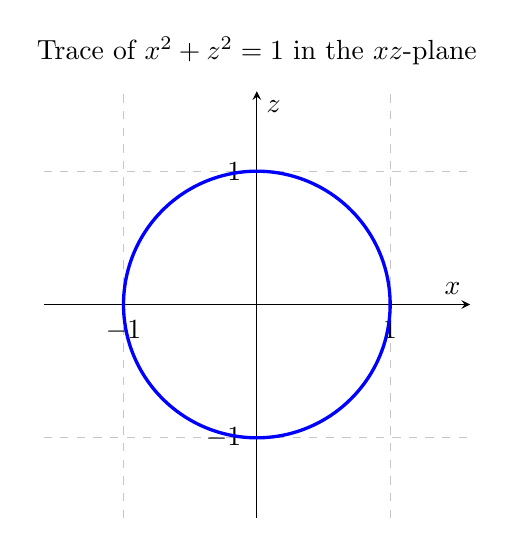
\begin{tikzpicture}
\begin{axis}[
    axis lines=center,
    xlabel={$x$},
    ylabel={$z$},
    axis equal,
    grid=both,
    grid style={dashed,gray!45},
    xmin=-1.6, xmax=1.6,
    ymin=-1.6, ymax=1.6,
    width=7cm,
    height=7cm,
    title={Trace of $x^2+z^2=1$ in the $xz$-plane}
]
\addplot[blue, very thick, domain=0:360, samples=200]
    ({cos(x)}, {sin(x)});
\end{axis}
\end{tikzpicture}
\end{document}